\section*{Discrete model}
%Хорда описана ломаной линией из элементов первого порядка, 
Investigating motion of any mechanical system comes to integration motion
equation of discrete parts of this system. Chordae tindae presents itself as
fibrous tissue and could be described as system of 1D rods, in case of getting
mechanical equivalent of system. Example of such flat 2D system are shown on
figure \ref{fig:nodeExtract}.
\begin{figure}[H]\label{fig:rodSystem}
  \centering
  \includesvg[width=0.8\columnwidth]{fig/systemAtworld}
  \caption{1D Rod system in global coordinate system}
\end{figure}
System consists of discrete elements $e_1$, $e_2$ and $e_3$. All elements are
connected to each other through nodes $n_2$, $n_3$ and to special points through
$n_1$ and $n_4$. Each element $e_n$ of system has own orientation in global
coordinate system. 
From schematic representation of node comes that all vector variables of node should be calculated
in global coordinate system and element variables in own local coordinate system(figure
\ref{fig:nodeExtract}). For transformation between coordinate systems direction cosine matrix
(DCM)\eqref{eqn:DCM} can be used.
\begin{equation}\label{eqn:DCM}
  DCM= \begin{bmatrix}
    cos(X,x) & cos(X,y) & cos(X,z) \\
    cos(Y,x) & cos(Y,y) & cos(Y,z) \\
    cos(Z,x) & cos(Z,y) & cos(Z,z) \\
  \end{bmatrix}
\end{equation}
where $\{X, Y, Z\}$ is global coordinate system and $\{x,y,z\}$ is local coordinate
system.\par According to primitive scheme of node \ref{fig:nodeExtract}, mass of
each node can be calculated, like sum of half mass of each element, which acting
in node. $m_n=\sum_{e}m_e/2$\par
In case that node does not have external interrupt, like pressure or other
applied force, schematic represent of node can be as on figure
\ref{fig:nodeExtract}.\par
\begin{figure}[H]
  \centering
  \includesvg[width=0.6\columnwidth]{fig/nodeExtract}
  \caption{Extracted node from system}\label{fig:nodeExtract}
\end{figure}
Mathematical model of discrete system is expressed by equations of nodes motion.
All system acting in global coordinate system $\{X, Y, Z\}$ and each element acting
in own local coordinate system $\{x,y,z\}$.

%В расчете целого клапана берется один стержень, существующие варианты расчетов всей системы и как в них рассчитывается хорда
\begin{figure}[H]\label{fig:pc1}
  \centering
  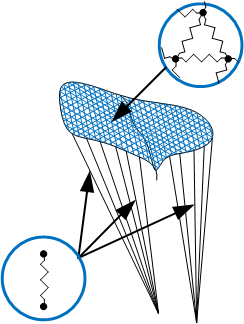
\includegraphics[width=0.35\columnwidth]{./fig/pc1.png}
  \caption{Displacement of papillary muscle over cardiac cycle}
\end{figure}
\begin{figure}[H]\label{fig:pc2}
  \centering
  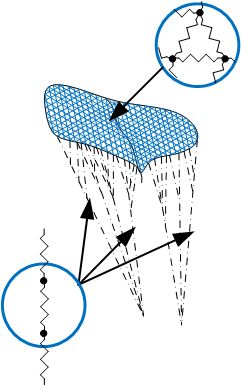
\includegraphics[width=0.35\columnwidth]{./fig/pc2.png}
  \caption{Displacement of papillary muscle over cardiac cycle}
\end{figure}
\begin{figure}[H]\label{fig:pc3}
  \centering
  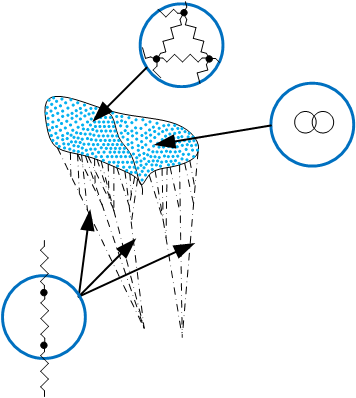
\includegraphics[width=0.45\columnwidth]{./fig/pc3.png}
  \caption{Displacement of papillary muscle over cardiac cycle}
\end{figure}
\cm{research aim is to compare 1 rod and rope of rods}
%Понятие линейной деформации, допущения, понятия и эфекты
%Движение узлов 
%Описать силы в узлах от стержней
%Учет напрвления элементов
If express $kx$ and $c\dot{x}$ by $\sum{F_{elem}}$,  then motion equantion will
become to:
\begin{equation}\label{eqn:sumF}
  \vec{F}_{inertia}= \vec{F}_{ext} - \sum\vec{F}_{elem}
\end{equation}
$F_{ext}$ is external load force, applied to node in global coordinates. Value
of this force for each time step is loaded from list of loads. $F_{elem}$ is sum
of internal forces of each element, which acting in node. From each element
counts only half of force to node, other half going to neighbour node.
For 1D rod system $F_{elem}$ can be expressed like:
\begin{equation}\label{eqn:Felem}
  F_{elem} = \sum_{e}N_e(x)
\end{equation}
To words about mechanical properties of valve components, poisson ratio $\nu$ is same, 0.49 for all.
Mean value of chordae length $L ~ 0,025 m$ and diameter $d ~ 0,001 m$. Chordae has density $\rho$
= 1040 kg/m3 and stiffness $E = 2000 N/m$, when leaflets has $\rho$ = 1.06E3 kg/m3 and 
$E = 2 MPa$ (Anterior leaflet), $E = 1 MPa$ (Posterior leaflet)\par